\section{Methodik}
\label{sec:methodik}

Die vorliegende Bachelorarbeit beschäftigt sich mit der Dekodierung verschiedener Dreiecksnetze mittels dem Kodierungstandard Brotli-G.
Diese Methodiksektion dient dazu, einen detaillierten Einblick auf die Durchführung und Analyse des Experiments zu geben.
Das Experiment zielt darauf ab, komprimierte Dreiecksnetze auf der GPU zu dekomprimieren.
Insbesondere sollen das Kompressionsverhältnis, Dekompressionsgeschwindigkeit und die visuelle Qualität quantitativ ausgewertet werden.

\subsection{Ablauf des Experiments}
\label{subsec:ablauf}
In diesem Abschnitt folgt eine kleine Beschreibung, wie die Kompressionspipeline aussieht.
In den Folgenden Kapiteln werden die einzelnen Teilschritte genauer erläutert. \newline
Zu Beginn muss der Datensatz mittels Brotli-G kodiert werden.
Der Einfachheit halber wird in diesem Abschnitt von einem einzigen Dreiecksnetz gesprochen.
Der Meshoptimizer von Zeux \cite{Zeux} ist dafür verantwortlich, aus den Positionen und Indizes die Meshletdaten zu generieren.
Dazu wurde ein Binärformat entworfen, welches die relevanten Daten zum Darstellen des gesamten Dreiecksnetzes speichert.
Das Binärformat besteht dementsprechend aus dem Meshlet Descriptor, Vertex Ressourcen (Positionen und Normalen) und den Indizes zur Primitivengenerierung. \newline
Dieses Binärformat wird als gesamtes komprimiert.
Anschließend werden die GPU Resourcen für die Eingabe (komprimiertes Dreiecksnetz) und Ausgabe (dekomprimiertes Dreiecksnetz) angelegt. \newline
Für die Ausgabe wird eine \glqq Unordered Acces View (UAV)\grqq\ verwendet.
Wie der Name schon vermuten lässt, bietet diese eine flexiblere Möglichkeit, gleichzeitig an verschiedenen Orten zu lesen und schreiben.
Besonders von Vorteil ist dieser Ressourcentyp für die parallele Verarbeitung.
So können einzelne Threads von der Ressource lesen/schreiben, ohne warten zu müssen, bis ein anderer Thread die Ressource wieder freigibt \cite{Microsoft2021}. \newline
Die UAV wird im Compute Shader als Output Buffer gesetzt, und mit den dekomprimierten Daten des Dreiecksnetzes gefüllt.

Abschließend wird die UAV im Mesh Shader gesetzt und die Meshlets und somit das gesamte Dreiecksnetz werden aus den Binärdaten rekonstruiert. \newline
Der gesamte Vorgang ist in Abbildung~\ref{fig:projekt} zu sehen.

\begin{figure}[htb]
  \centering  
  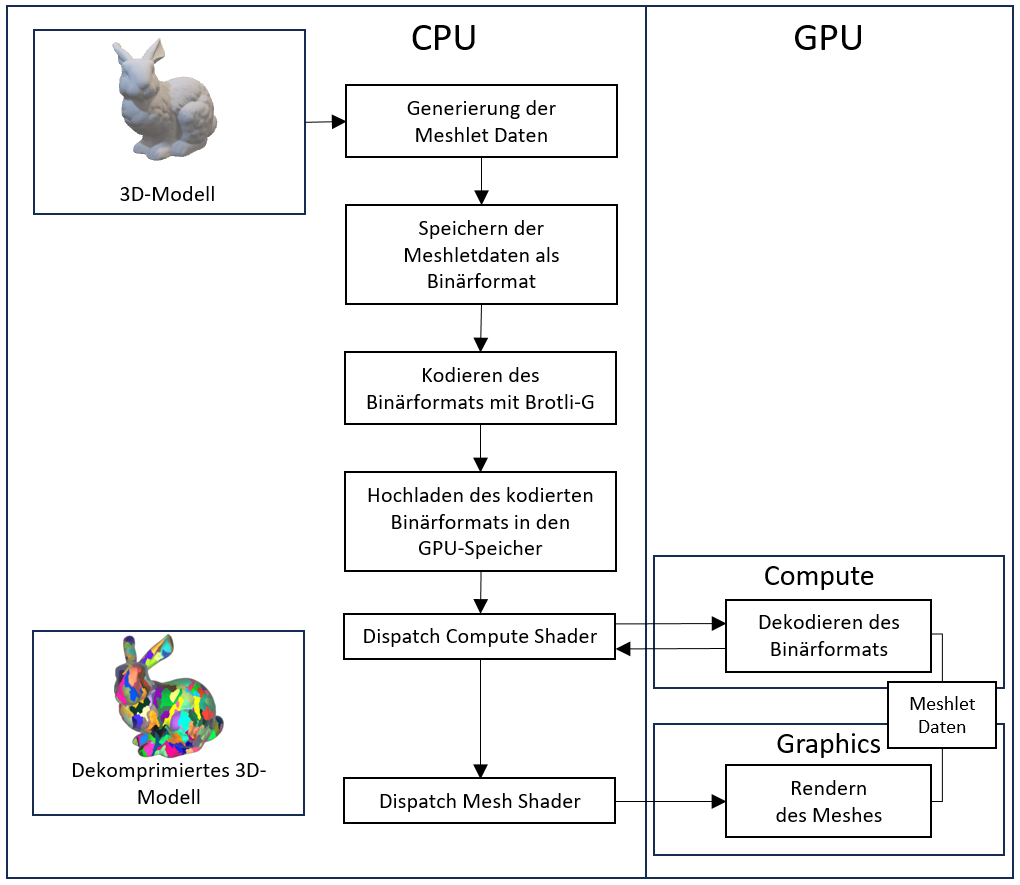
\includegraphics[scale=0.6]{Bilder/Ablauf_Projekt.png}
  \caption[Flussdiagramm Ablauf]{\textbf{Flussdiagramm Ablauf} Abbildung der Dekompressionspipeline.}
  \label{fig:projekt}
\end{figure}

Ist dieser Schritt abgeschlossen, könnten die Daten der UAV auf der CPU ausgelesen werden, die Buffer der Mesh Shader verwendet gefüllt werden und in den GPU RAM geschrieben werden.
Dieser Schritt ist jedoch als unnötig anzusehen, wenn nicht noch zusätzliche Informationen mit dem dekomprimierten Dreiecksnetz berechnet werden müssen.
Der Output Buffer des Brotli-G Dekodierers beinhaltet schon die benötigten Meshlet Daten, um das Dreiecksnetz zu rekonstruieren.
So kann ein GPU Buffer außerhalb von Brotli-G angelegt werden, den Brotli-G als Output Buffer verwendet.
Dadurch wird dieser Buffer nicht freigegeben, nachdem der Dekompressionsschritt von Brotli-G abgeschlossen ist.
Abschließend übergibt man dem Mesh Shader den Output Daten Buffer und kann aus diesem das Dreiecksnetz rekonstruieren.

\subsection{Mesh Shader}
\label{susbsec:mesh_shader}
